\documentclass[12pt, %
openright, 
oneside, %
%twoside, %TCC: Se seu texto tem mais de 100 páginas, descomente esta linha e comente a anterior
a4paper,    %
%english,   %
brazil]{facom-ufu-abntex2}
\usepackage{xcolor}
% Definindo novas cores
\definecolor{verde}{rgb}{0.25,0.5,0.35}
\definecolor{jpurple}{rgb}{0.5,0,0.35}
% Configurando layout para mostrar codigos Java
\usepackage{listings}
\lstset{
  language=Java,
  basicstyle=\ttfamily\small, 
  keywordstyle=\color{jpurple}\bfseries,
  stringstyle=\color{red},
  commentstyle=\color{verde},
  morecomment=[s][\color{blue}]{/**}{*/},
  extendedchars=true, 
  showspaces=false, 
  showstringspaces=false, 
  numbers=left,
  numberstyle=\tiny,
  breaklines=true, 
  backgroundcolor=\color{cyan!10}, 
  breakautoindent=true, 
  captionpos=b,
  xleftmargin=0pt,
  tabsize=4
}
\autor{Patrick Godinho} %TCC
\data{2014}
\orientador{Lásaro Camargos} %TCC
%\coorientador{Algum?} %TCC 


% ---
% Informações de dados para CAPA e FOLHA DE ROSTO
% ---

\titulo{PheroCast App} %TCC

\hypersetup{pdfkeywords={palavra 1}{palavra 2}{palavra 4}{palavra 4}{palavra 5}} %TCC

\begin{document}
\frenchspacing 

% ----------------------------------------------------------
% ELEMENTOS PRÉ-TEXTUAIS
% ----------------------------------------------------------
%\pretextual
\imprimircapa
\imprimirfolhaderosto


% ---
% Inserir folha de aprovação
% ---
%
% \includepdf{folhadeaprovacao_final.png} %TCC: depois de aprovado o trabalho, descomente esta linha e comente o próximo bloco para incluir scan da folha de aprovação.
%
\begin{folhadeaprovacao}

  \begin{center}
    {\ABNTEXchapterfont\large\imprimirautor}

    \vspace*{\fill}\vspace*{\fill}
    {\ABNTEXchapterfont\bfseries\Large\imprimirtitulo}
    \vspace*{\fill}
    
    \hspace{.45\textwidth}
    \begin{minipage}{.5\textwidth}
        \imprimirpreambulo
    \end{minipage}%
    \vspace*{\fill}
   \end{center}
    
   Trabalho aprovado. \imprimirlocal, 24 de novembro de 2012: %TCC:

   \assinatura{\textbf{\imprimirorientador} \\ Orientador}  
   \assinatura{\textbf{Faina}}% \\ Convidado 1} %TCC:
   \assinatura{\textbf{Professor}}% \\ Convidado 2} %TCC:
   %\assinatura{\textbf{Professor} \\ Convidado 3}
   %\assinatura{\textbf{Professor} \\ Convidado 4}
      
   \begin{center}
    \vspace*{0.5cm}
    {\large\imprimirlocal}
    \par
    {\large\imprimirdata}
    \vspace*{1cm}
  \end{center}
  
\end{folhadeaprovacao}
% ---


%%As seções dedicatória, agradecimento e epígrafe não são obrigatórias.
%%Só as mantenha se achar pertinente.

% ---
% Dedicatória
% ---
\begin{dedicatoria}
   \vspace*{\fill}
   \centering
   \noindent
   \textit{Dedico a meu pai Paulo Sergio de Jesus Oliveira que sempre foi um exemplo de perseverança na minha vida!}  %TCC:
   \vspace*{\fill}
\end{dedicatoria}
% ---

% ---
% Agradecimentos
% ---
\begin{agradecimentos}
Agradeço a Deus, minha esposa e ao meu orientador pelo apoio e dedicação para que eu conseguisse chegar ao final deste trabalho. %TCC:
\end{agradecimentos}
% ---

% ---
% Epígrafe
% ---
\begin{epigrafe}
    \vspace*{\fill}
	\begin{flushright}
		\textit{``Alguma citação que ache conveniente? \lipsum[10]''} %TCC:
	\end{flushright}
\end{epigrafe}
% ---



\begin{resumo} %TCC:
 o resumo deve ressaltar o teste
 objetivo, o método, os resultados e as conclusões do documento. A ordem e a extensão
 destes itens dependem do tipo de resumo (informativo ou indicativo) e do
 tratamento que cada item recebe no documento original. O resumo deve ser
 precedido da referência do documento, com exceção do resumo inserido no
 próprio documento. (\ldots) As palavras-chave devem figurar logo abaixo do
 resumo, antecedidas da expressão Palavras-chave:, separadas entre si por
 ponto e finalizadas também por ponto. teste teste

 \vspace{\onelineskip}
    
 \noindent
 \textbf{Palavras-chave}: Manet, Android, Redes Oportunísticas%TCC:
\end{resumo}

% ---
% inserir lista de ilustrações
% ---
\pdfbookmark[0]{\listfigurename}{lof}
\listoffigures*
\cleardoublepage
% ---

% ---
% inserir lista de tabelas
% ---
\pdfbookmark[0]{\listtablename}{lot}
\listoftables*
\cleardoublepage
% ---



% ---
% inserir lista de abreviaturas e siglas
% ---
\begin{siglas} %TCC:
  \item[Fig.] Area of the $i^{th}$ component
  \item[456] Isto é um número
  \item[123] Isto é outro número
  \item[Zézão] este é o meu nome
\end{siglas}
% ---

%% ---
%% inserir lista de símbolos, se for adequado ao trabalho. %TCC:
%% ---
%\begin{simbolos}
%  \item[$ \Gamma $] Letra grega Gama
%  \item[$ \Lambda $] Lambda
%  \item[$ \zeta $] Letra grega minúscula zeta
%  \item[$ \in $] Pertence
%\end{simbolos}
%% ---

% ---
% inserir o sumario
% ---
\pdfbookmark[0]{\contentsname}{toc}
\tableofcontents*
\cleardoublepage
% ---





% ----------------------------------------------------------
% ELEMENTOS TEXTUAIS
% ----------------------------------------------------------
\textual


% ----------------------------------------------------------
% Introdução
% ----------------------------------------------------------

\chapter{Introdução}
\addcontentsline{toc}{chapter}{Introdução}
%TCC:
\section{Contextualização}
O paradigma dos multiplos saltos (\emph{multihop}) das redes mobile MANET (Mobile Ad hoc Networking) surgiu no campo da civilização nos anos 90 com a disponibilização das tecnologias wireless de prateleira capazes de fornecer conexões diretas entre os usuários de dispositivos, como por exemplo o Bluetooth(IEEE 802.15.1) para redes pessoais, e a 802.11 standards family para redes de alta velocidade. Especificamente esses padrões de rede sem fio permitiam comunicação direta entre os dispositivos de rede, na faixa de transmissão de suas interfaces sem fio, tornando a rede "single-hop ad hoc" uma realidade, isto é, "WLAN/WPAN infraestructureless" onde dispositivos comunicam sem a necessidade de nenhuma infraestrutura de rede.



Desde que surgiu, a MANET tem sido visto como um dos mais inovadores e desafiantes paradigmas de redes sem fio, e prometia tornar-se uma das principais tecnologias, cada vez mais presente no cotidiano de todos. As potencialidades desse paradigma de rede fez a rede ad-hoc uma opção atrativa para a construção das redes sem fio 4G, e portanto a MANET imediatamente ganhou impulso, e isto produziu enormes esforços de pesquisa na comunidade de redes móveis. 

Ao passar dos anos a MANET sofreu  com o pouco interesse e exploração das indústrias e entre os usuários[8]. Tal fato pode ser explicado por algumas razões tais como a alta complexidade da implementação, integração e experimentação; a falta de credibilidade nas simulações, e a baixa motivação socio-econômica para com essa tecnologia.

Impulssionados pelas lições aprendidas com a MANET, surgiram algumas Redes Móveis com a promessa de evitar os erros cometidos anteriormente seguindo uma abordagem de desenvolvimento mais pragmática, desenvolvendo orientado a aplicações, com redução de complexidade, com uma abordagem de pesquisa voltada ao cenário da aplicação, utilizando o modelo de simulação realista, a fim de basear o desenvolvimento do protocolo em estudos de simulações confiáveis e acreditáveis; e O desenvolver os testes de mesa reais com a participação de usuários, nos estágios iniciais do projeto desses novos paradigmas, a fim de colocar esses usuários envolvidos com o projeto da rede e testes de experimentação.\cite{6710069}

Dentre esses paradimas de rede que surgiram destacaremos a Rede Oportunística a qual não considera a mobilidade dos nós um problema, e sim uma oportunidade de ser explorada,ou seja, nesse paradigma a mobilidade dos nós cria oportunidades de contato entre os mesmos, sendo assim, entender e modelar as propriedades da mobilidade humana, bem como o tempo em que dois dispositivos ficam conectados, ou o tempo para que crie outra comunicação, é fundamental para caracterizar as restrições das comunicações oportunísitcas.
asd
Outra rede que terá destaque na fundamentação teórica deste trabalho são as Redes Veículares criadas para veículos que comunicam entre si explorando tecnologias sem fio. A VANET pode suportar uma plenitude de aplicações como de segurança veicular, propagação de tráfego, compartilhamento de entretenimento e dentre outras.

Estudar os rastros da movimentação humana, é o ponto de partida para entender as propriedades da mobilidade, com o objetivo de fornecer as características temporais da mobilidade dos dispositivos/usuários. Experiências que são também usadas para derivar modelos de mobilidade, que são a base para simulações de rede oportunistas realistas. Além de estudos que tentam acoplar os resultados com os aspectos sociais dos donos dos dispositivos. \cite{6838650}

Esse trabalho tem como objetivo desenvolver uma aplicativo Android para a coleta de dados sobre a mobilidade de usuários de smartphones, o qual coletará pontos de redes sem fio que seus dispositivos encontrarem durante seu dia-a-dia, ou seja, deixará registrado que passou em determinado ponto de rede.Após a coleta, armazenará nas nuvens para uma possível análise 
realista da mobilidade do usuário.

O aplicativo foi nomeado PheroCast App, por ser um trabalho impulssionado tambem para a cooperação para a pesquisa do PheroCast, algoritmos para prever a posição futura de nós móveis em MANET, permitindo que as infra-estruturas se adaptem de forma proactiva. Algoritmos estes denominados PheroCast, nome dado pela inspiração ao fenômeno que acontece na comunidade de formigas, em que a troca de informações acontece através da deposição e detecção de feromônios no ambiente.
\cite{6838650}


Após coleta dos dados, iremos contribuir com a \emph{Crawdad}, um projeto de pesquisa em redes sem fio, a qual demandam logs e dados capturados através de redes \emph{wireless}, para o estudo de como usuários reais, aplicações e dispositivos usam redes reais sob condições reais. Nossos dados cooperarão para enteder problemas, possiveis soluções e avaliar novas aplicações e serviços.



\chapter{Fundamentação Teórica}
\section{Redes Móveis}
\subsection{MANET}
O paradigma dos multiplos saltos (\emph{multihop}) das redes mobile MANET (Mobile Ad hoc Networking) surgiu no campo da civilização nos anos 90 com a disponibilização das tecnologias wireless de prateleira capazes de fornecer conexões diretas entre os usuários de dispositivos, como por exemplo o Bluetooth(IEEE 802.15.1) para redes pessoais, e a 802.11 standards family para redes de alta velocidade. Especificamente esses padrões de rede sem fio permitiam comunicação direta entre os dispositivos de rede, na faixa de transmissão de suas interfaces sem fio, tornando a rede "single-hop ad hoc" uma realidade, isto é, WLAN/WPAN infraestructureless" onde dispositivos comunicam sem a necessidade de nenhuma infraestrutura de rede.
O paradigma multihop foi então idealizado para tornar possível a comunicação entre 2 nós de rede, sem a necessidade de desenvolver nenhuma  infraestrutura de rede onipresente. Nos anos 90, temos assistido a utilização do paradigma "multihop" nas  MANETs (Redes ad-hoc móveis) onde usuários próximos (fisicamente) comunicam diretamente entre si (explorando as interfaces de redes sem fio de seus dispositivos no modo ad-hoc) não apenas para compartilhar seus dados, mas tambem para retransmitir o trafico de outros pontos de rede que não podem comunicar diretamente, operando assim como os roteadores fazem na internet. Por essa razão. na MANET, dispositivos dos usuários cooperativamente podem fornecer serviço de internet, geralmente fornecida pela rede de infra-estrutura (por exemplo, roteadores, switches, servidores).
Desde que surgiu, a MANET tem sido visto como um dos mais inovadores e desafiantes paradigmas de redes sem fio, e prometia tornar-se uma das principais tecnologias, cada vez mais presente no cotidiano de todos. As potencialidades desse paradigma de rede fez a rede ad-hoc uma opção atrativa para a construção das redes sem fio 4G, e portanto a MANET imediatamente ganhou impulso, e isto produziu enormes esforços de pesquisa na comunidade de redes móveis.
O modelo INTERNET foi a central para a MANET Internet Engineering Task Force (IETF) grupo de trabalho, o qual, herdou os protocolos TCP/IP stack layering, assumindo a visão do MANET centrada em IP. see “Mobile Ad Hoc
Networks (MANETs)” by J. P. Macker and M.
S. Scott Corson in [1].
As pesquisas da comunidade MANET tem sido focadas no que chamamos de de "pure general purpose MANETs" (objetivo geral puro), onde o "puro" indica que não há infrastrutura para implementar as funcionalidades de rede, e nenhuma autoridade é responsável para gerenciar e controlar a rede. 

\subsection{Redes Oportunísticas}
Redes Oportunisticas é uma das mais interessantes evoluções do paradigma de rede baseada em saltos (multihop). De fato, enquanto MANET representa uma abordagem para esconder a mobilidade dos nós construindo um estável caminho fim a fim como na Internet, redes oportunísticas não consideram a mobilidade dos nós um problema, e sim uma oportunidade de ser explorada. Nas Redes Oportunísticas, a mobilidade dos nós cria oportunidades de contato entre os mesmos, as quais podem ser usadas por exemplo para conectar partes de redes que são de outra forma desconectada. Especificamente, de acordo com esse paradigma, nós podem carregar fisicamente dados em seu buffer enquanto eles se movimentam na rede, até que eles entrem em contato com um adequado ad-hoc. Assim, ao contrário da MANET, um nó mantem o armazenamento do dado enquanto não há um proximo bom salto "hop". Isso implica que, com o paradigma oportunistico, um dado pode ser entregue de uma origem para um destino mesmo se não existir um caminho fim-a-fim entre eles, explorando a sequência de gráficos gerados pela movimentação dos nós. [33,34]. Esse é um paradigma relativamente jovem, e a pesquisa da rede oportuniística ainda está ocorrendo. Entretanto, pode se argumentar que seu impacto ainda será provado. No entanto, dado que podemos considerar a rede ad-hoc veicular (VANET), uma dos mais avançados e concretos desenvolvimentos do paradigma das redes oportunísticas, podemos afirmar que esse paradigma já tem um papel significativo na área de redes de computadores.
Além da VANET, outros cenários motivam a rede oportunística, discutido em [7]. Redes Oportunísticas, rede oportunísticas parecem muito adequadas para comunicações 
em ambientes difusos onde o ambiente está saturado por dispositivos (com tecnologias sem fio de curto alcance) que podem se auto-organizar em uma rede de interações locais entre os usuários. Nesses cenários, a rede é geralmente dividida em ilhas desconectadas, o que pode ser interligados explorando a mobilidade dos nós. Isso implica em uma mudança da comunicação baseada em pacotes, para comunicação baseada em mensagens, trazendo novas oportunidades para o desengo do protocolo das aplicações. 

Rede Oportunistica se afasta da abordagem orientada a Internet utilizada na MANET, pois não prevê um caminho fim-a-fim da origem para o destino. Isso elimina o grande esforço de esconder a mobilidade dos nós, tal fato que causou a complexidade alta nas MANETs. Na Rede Oportunística, o paradigma "multihop" se torna mais eficiente, pelo fato de não necessitar manter caminhos e tabelas de rotas), e a mobilidade dos humanos torna uma oportunidade de comunicação.

Três principais direções tem caracterizado a pesqusia em rede oportunística, modelos de mobilidade, protocolos de roteamento e disseminação de dados.

Entender e modelar as propriedades da mobilidade humana, é fundamental para caracterizar as restrições das comunicações oportunísitcas, e desenhar as eficientes e práticas estratégias de compartilhamento[35,36]. Os principais elementos que caracterizam a mobilidade humana é o "contact time", que se dá pela duração entre dois dispositivos; e o "inter-contact time" (ICT) que se dá pela duração entre dois contatos consecutivos entre dispositivos. Em particular, a caracterização da ICT tem gerado um excelente debate na comunidade científica as quais diferentes grupos de pesquisa têm reportado diferentes resultados variando entre várias funções.
\subsection{VANET}

A Rede Veicular AdHoc (VANET) é uma rede "multihop" adhoc criada para veículos que comunicam entre si explorando tecnologias sem fio (tipicamente) pertencentes a família 802.11. Essa é uma especialização do paradigma "multihop" adhoc bem mtivado pelo valor sócio-econômico dos avançados Sistemas de Transporte Inteligente (ITS) destinados a reduzir os congestionamentos, o número de acidentes, dentre outros. De fato, VANET pode suportar uma plenitude de aplicações incluindo as que envolvem segurança no tráfego (alertas de obstáculos na estrada, disseminação de mensagens de segurança), informações de tráfego e serviços de entretenimento/informações(jogos, streaming de multimedia, dentre outros). Um outro exemplo é um carro envolvido em um acidente pode explorar a possibilidade de se comunicar diretamente com outros veículos para informar os veículos próximos da situação perigosa.[44]

Sistemas ITS avançados necessitam tanto de comunicações vehicle-to-roadside (V2R) tanto como as vehicle-to-vehicle (V2V). Nas comunicações V2R um veículo tipicamente explora tecnologias sem fio baseada em infra-estrutura, como redes de celular, WiMAX e Wi-Fi, para comunicar com um ponto de estação ou acesso da estrada. No entanto, as unidades da estrada não são densas o suficiente para garantir a cobertura de rede exigido pelas aplicações e, portanto, são adotadas as comunicações V2V para estender a conectividade de rede/cobertura e garantir melhor desempenho da rede. 

Comunicações V2V são baseadas no paradigma de rede multihop ad hoc "puro" como no MANET. Especificamente, de acordo com esse paradigma, os veículos na estrada se auto organizam dinamicamente na VANET explorando suas interfaces de comunicação sem fio. No entanto, o alto nível de mobilidade e a possibilidade do cenário de escassez de rede causadas pela baixa intensidade do tráfico, torna ineficiente o paradigma de comunicação utilizado na MANET "store-and-forward" utilizado na MANET, e força para a adoção do mais flexível, pragmático e robusto "store-carry-and-forward" paradigma, adotado pelas redes oportunísticas.

Além disso, sempre que possível as comunicações V2V exploram as comunicações V2R para se tornarem mais robustas e reduzindo algumas fragilidades e vulnerabilidades de uma comunicação "infrastructureless" pura.

O Alto valor socio-econômico das aplicações veiculares impulssionaram as organizações internacionais de normalização para elaborar especificações técnicas a serem adotadas pela indústria de veículos. Entre eles, vale a pena lembrar a família padrão IEEE 1609 para acesso wireless em Ambiente Veicular(WAVE), que foi desenvolvido com base no padrão IEEE 802.11p. Normalmente, o consumo de energia não é um problema para esta rede como 
baterias para veículos são continuamente recarregado.

Comunicações V2R exploram tecnologias bem estabelecidas (Wi-Fi, WiMAX, ZigBee, etc) que operam baseados em infra-estrutura. Sua adoção em redes veiculares requer uma análise cuidadosa de seu desempenho ao operar em ambientes altamente dinâmicos, onde o tempo de conexão entre o veículo e a unidade na estrada pode ser curto e/ou vários veículos estão conectados à mesma unidade de beira de estrada (questão escalabilidade).

O campo de pesquisa em V2V herdaram resultados obtidos em MANET relacionados aos protocolos de roteamento/compartilhamento multihop ad hoc, os quais tem sido melhorado e modificado para adaptar-los as peculiaridades da área veicular. A tarefa de roteamento é um desafio na VANET, devida à alta mobilidade dos veículos que são conectados entre si intermitentemente.
Entretanto, em VANET, a mobilidade dos pontos de redes (veiculos) são restritos pelas caracteristicas da estrada, e pelos outros veiculos que movimentam ao longo da estrada. Uma atenção especial está sendo reservada para o desenvolvimento dos otimizados "one-to-all" protocolos de roteamento assim como várias aplicações desenvolvidas para VANET usam comunicações broadcasting (geocasting). Broadcast ou geocast são tambem os serviços basicos de comunicação para disseminação de conteudo na VANET. Devida as alternadas condições de conectividade, o paradigma oportunístico aplicado a rede veicular tem gerado recentemente uma grande quantidade de literaturas, principalmente em protocolos de roteamento e disseminação de dados nas redes veiculares.

Tanto simulação quanto experimentos tem papéis importantes na formulação e avaliação das soluções desenvolvidas para redes veiculares. Nas simulações das redes veiculares, bastante atenção tem sido dedicado para desenvolver modelos realistas de estradas e de mobilidade dos veículos através do estudo e aprofundamento de literaturas desenvolvidas na área de sistemas de transporte, por exemplo modelos de como os carros se movem ao longo de uma estrada, tendo em conta a sua velocidade, a distância entre eles, sinais de trânsito, o traçado viário, etc

Um aspecto importante para se considerar está relacionado à simulação dos canais sem fio entre veículos e de/para unidades na estrada levando em conta a forma como o sinal de rádio propaga neste ambiente.

\section{Desenvolvimento para Smartphones}

Com o grande progresso da produção e comercialização de smartphones e tablets (e.g., Applet Ipad, Apple Iphone, Galaxy S4), fica evidente a quantidade de pessoas que foram alcançadas pelos dispositivos móeis, em especial pelos smartphones. Nota-se que existe, de fato, uma grande migração da computação tradicional, baseada em computadores pessoais, para uma nova era, muitas vezes chamadas de computação ubíqua.

 A idéia desse novo paradigma, em geral, é expor um novo mundo, onde a computação está totalmente inserida e acoplada no cotidiano da vida das pessoas, principalmente a partir do uso de dispositivos que comunicam-se de forma transparente, possibilitando a troca de informações em qualquer momento e em qualquer lugar.

Levando isto em conta, é notável e fundamental, o desenvolvimento de novos sistemas operacionais e aplicações que atendam essa área em um crescente avanço e evolução. Tais aplicações que se diferenciam dos presentes na computação tradicional (i.e.. aplicações desktop), como por exemplo a substituição dos meios de entrada de dados, que se dava por teclado e mouse, por algo mais intuitivo como a utilização de telas sensíveis ao toque.

O mercado corporativo também está crescendo muito, e diversas empresas estão buscando incorporar aplicações móveis a seu dia-a-dia para agilizar seus negócios e integrar as aplicações móveis com seus sistemas de back-end. Empresas obviamente visam lucro e mais lucro, e aos celulares e smartphones podem ocupar um importante espaço em um mundo onde a palavra "mobilidade" está cada vez mais conhecida.[unijui]


Desta forma aplicações que executam em um celular podem estar literalmente conectadas e online, sincronizando informações diretamente de um servidor confiável da empresa. Hoje em dia diversos bancos oferecem serviços aos seus usuários, onde é possível pagar suas contas e visualizar o extrato de sua conta corrente diretamente de um celular.

As empresas e os desenvolvedores buscam uma plataforma moderna e ágil para o desenvolvimento de aplicações para auxiliar em seus negócios e lucros. Já os usuários comuns buscam um celular ocm um visual elegante e moderno, de fácil navegaão e uma infinidade de recursos.

Para acompanhar essa evolução da tecnologia e satisfazer os usuários, os fabricantes e operadoras de celulares, as empresas e os desenvolvedores, existe uma grande corrida estrelada pelas maiores empresas do mundo em tecnologia móvel para competir por esse nicho do mercado.\cite{googleand}




\subsection{Android}
O Android é uma plataforma de desenvolvimento para aplicativos móveis, baseada em um sistema operacional Linux, uma interface visual rica, diversas aplicações já instaladas e ainda um ambiente de desenvolvimento bastante poderoso, inovador e flexível. Outro ponto importante é a possibilidade de utilizar a linguagem Java para desenvolver aplicações usufruindo de todos os recursos que a poderosa linguagem fornece. Entretanto possui suportepara o desenvolvimento de aplicações nativas, escritas em C e C++, através do android NDK. \cite{googleand}

A primeira plataforma para aplicações móveis completamente livre e de código aberto (open-source) foi o Android, o que representa uma grande vantagem para sua evolução, uma vez que diversos programadores do mundo poderão contribuir para melhorar a plataforma. Tais características, cooperaram para a escolha pelo Android a nossa plataforma de desenvolvimento do aplicativo deste trabalho.

Com a variedade de recursos do Android, seria fácil confundi-lo com um sistema operacional desktop. O Android é um ambiente em camadas baseado em kernel Linux e que inclui funções ricas. O subsistema da UI inclui:
\begin{itemize}
\item Janelas
\item Visualizações
\item Widgets para a exibição de elementos comuns como caixas de edição, listas e listas suspensas
\end{itemize}


O Android inclui um navegador incorporável baseado em WebKit, o mesmo mecanismo navegador de software livre equipando o navegador Mobile Safari do iPhone.

O Android ostenta uma rica lista de opções de conectividade, incluindo WiFi, Bluetooth e dados wireless através de uma conexão celular (por exemplo, GPRS, EDGE e 3G). Uma técnica popular em aplicativos Android é estabelecer um link com o Google Maps para exibir um endereço diretamente em um aplicativo. O suporte para serviços baseados em locais (como GPS) e acelerômetros também está disponível na pilha de software Android, embora nem todos os dispositivos Android sejam equipados com o hardware necessário. Existe também suporte para câmera.

Historicamente, duas áreas onde aplicações móveis lutaram para acompanhar suas contrapartes de desktop são gráfico/mídia e métodos de armazenamento de dados. O Android aborda o desafio dos gráficos com suporte integrado para gráficos em 2-D e 3-D, incluindo a biblioteca OpenGL. O peso do armazenamento de dados é amenizado porque a plataforma Android inclui o banco de dados SQLite de software livre popular. A Figura 1 mostra uma visualização simplificada das camadas do software Android.

\begin{figure}[!htb]
    \centering
    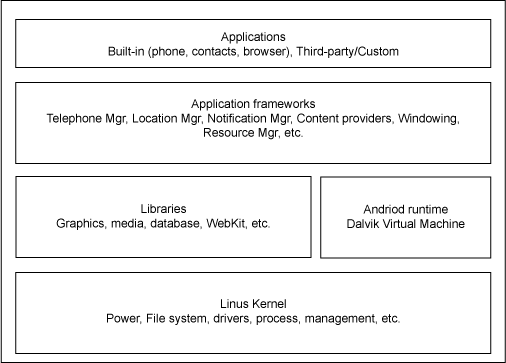
\includegraphics[scale=0.8,natwidth=610,natheight=64]{plataformas.png}
    \caption{Camadas do Software Android}
    \label{figRotulo}
  \end{figure}



Conforme mencionado, o Android é executado sobre um kernel Linux. Os aplicativos Android são gravados na linguagem de programação Java e são executados em uma máquina virtual (VM). É importante observar que a VM não é uma JVM, como você pode esperar, mas é uma Dalvik Virtual Machine, uma tecnologia de software livre. Cada aplicativo Android é executado em uma instância da Dalvik VM, que, por sua vez, reside em um processo gerenciado por kernel Linux, conforme mostrado abaixo.
\begin{figure}[!htb]
    \centering
    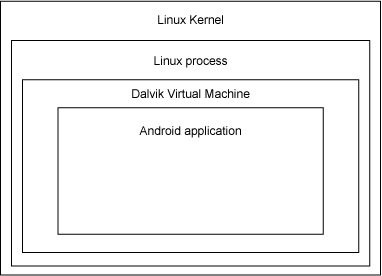
\includegraphics[scale=0.8,natwidth=610,natheight=64]{plataforma.png}
    \caption{Dalvik VM}
    \label{figRotulo}
  \end{figure}

Um aplicativo Android consiste em uma ou mais das classificações a seguir:

\textbf{Atividades}
Um aplicativo que possui uma UI visível é implementado com uma atividade. Quando um usuário seleciona um aplicativo da tela inicial ou de um ativador de aplicativo, uma atividade é iniciada.

\textbf{Serviços}
Um serviço deve ser utilizado para qualquer aplicativo que precise persistir por um longo período de tempo, como um monitor de rede ou um aplicativo de verificação de atualização.

\textbf{Provedores} de conteúdo
Você pode pensar em provedores de conteúdo como um servidor de banco de dados. O trabalho de um provedor de conteúdo é gerenciar o acesso aos dados que persistem, como um banco de dados SQLite. Se seu aplicativo for muito simples, você não precisa necessariamente criar um provedor de conteúdo. Se estiver construindo um aplicativo maior, ou um que disponibilize dados para várias atividades ou aplicativos, um provedor de conteúdo será o meio de você acessar seus dados.

\textbf{Receptores de transmissão}
Um aplicativo Android pode ser ativado para processar um elemento de dados ou para responder a um evento, como o recebimento de uma mensagem de texto.
Um aplicativo Android, junto com um arquivo chamado AndroidManifest.xml, é implementado em um dispositivo. O AndroidManifest.xml contém as informações de configuração necessárias para você instalá-lo corretamente no dispositivo.

 Ele inclui os nomes de classes necessários e os tipos de eventos que o aplicativo está pronto para processar, além das permissões necessárias que o aplicativo precisa para execução. Por exemplo, se um aplicativo exigir acesso à rede — para fazer o download de um arquivo, por exemplo — essa permissão deve ser declarada explicitamente no arquivo de manifesto. Muitos aplicativos podem ter essa permissão específica ativada. Tal segurança declarativa ajuda a reduzir a probabilidade de um aplicativo perigoso causar danos em seu dispositivo.\cite{IBM:Android}


%\chapter{Revisão Bibliográfica}
%TCC:

%Um ou mais capítulos (por exemplo, se há duas linhas de trabalhos relacionados.

\chapter{Desenvolvimento}
%TCC:
Este trabalho foi desenvolvido na linguagem Java orientado a objetos , utilizando o Android SDK integrado com a IDE Eclipse. 

Este trabalho se divide em três partes: 1- Execução periódica; 2- BroadCastReceiver - Coleta dos dados;3- Armazenamento na nuvem


\section{Execução periódica} 
Para coletar os dados, o aplicativo acorda a cada um minuto e uma thread é executada, a qual verifica se o serviço de WIFI está ligado no aparelho. Se sim, a thread registra um \emph{BroadCast Receiver} responsável por receber a lista de pontos de rede que estão ao alcance do dispositivo. Após receber a lista, é cancelado o registro do \emph{BroadCast Receiver}.
Caso o serviço de Wifi do celular esteja desligado, é feito o mesmo procedimento descrito acima, mas ligando o Wifi no começo da operação, e desligando no final, assim como está desenhado o diagrama abaixo.
\begin{figure}[!htb]
    \centering
    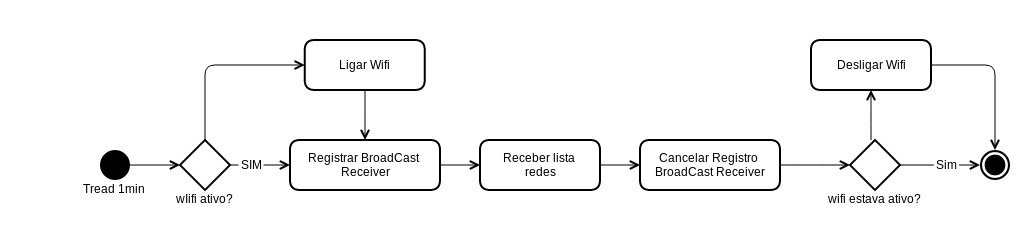
\includegraphics[scale=0.45,natwidth=610,natheight=64]{pherocast1.png}    \caption{Diagrama de estado de execução da thread}
    \label{figRotulo}
  \end{figure}

\section{BroadCastReceiver - Coleta dos dados}
No momento em que a lista de pontos de rede é recebida pelo BroadCastReceiver, para cada registro da lista é criado um objeto da classe NetworkPoint a qual possui os atributos da rede. Esses atributos são definidos pela classe nativa do Android \emph{ScanResult}, sendo eles:

\begin{itemize}
\item BSSID (MAC address)
\item SSID (Nome da rede)
\item capabilities (Características gerais)
\item frequency (Frequência)
\item level (Nível de distância)
\end{itemize}
Além desses atributos, também é guardado a hora em que o dispositivo passou pela rede.

Após criar o objeto, o mesmo é gravado no banco de dados local através das funções da classe NetworkPointDAO.
\begin{figure}[!htb]
    \centering
    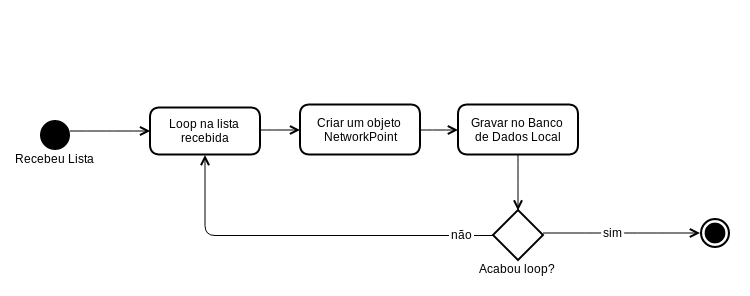
\includegraphics[scale=0.45,natwidth=610,natheight=64]{pherocast2.png}
    \caption{Diagrama de estado de execução do BroadCast Receiver}
    \label{figRotulo}
  \end{figure}
  
\section{Descarregando na nuvem}
No aplicativo, registramos um filtro a fim de sempre que o dispositivo conectar-se a internet pela tecnologia Wifi, um método que escrevemos para descarregar os dados armazenados na nuvem seja executado.
O armazenamento na nuvem foi feito através do mecanismo de formulário da plataforma Google Docs, onde fazemos requisições HTTP, como se estivéssemos respondendo ao formulário. Assim as respostas do mesmo são guardadas em uma planilha, a qual estão armazenados os campos do objeto mais o identificador do usuário, que no caso escolhemos o e-mail registrado no aparelho.
\begin{figure}[!htb]
    \centering
    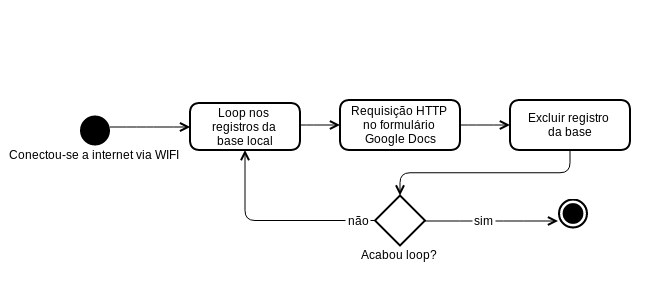
\includegraphics[scale=0.45,natwidth=610,natheight=64]{pherocast3.png}
    \caption{Diagrama de estado de execução do armazenamento na nuvem}
    \label{figRotulo}
  \end{figure}
%TCC:
%TCC:
%TCC:
%TCC:
\chapter{Resultados}
% ---
% Conclusão
% ---
\chapter*[Conclusão]{Conclusão e Trabalhos Futuros}
\addcontentsline{toc}{chapter}{Conclusão}
%TCC:

No decorrer do desenvolvimento deste trabalho, surgiram algumas idéias que foram consideradas como trabalhos futuros serem complementados. Por exemplo, implementar a anonimização dos dados, ou seja, para que cada usuário que cooperou com a coleta do log, não seja identificado. Tal requisito poderia ser implementado com o uso da teconologia GUID , a qual cria um identificador anônimo para cada dispositivo.

Concluímos no desenvolvimento do nosso trabalho que a escolha pela plataforma do Google Docs, apesar de ser uma maneira prática de armazenamento de dados, apresenta problemas de escabilidade dependendo da quantidade de dados a serem armazenados, pelo fato da exibição dos dados se dar através de planilhas. Uma sugestão para trabalhos futuros seria a implementação de um serviço próprio para captação e armazenamento de dados, como por exemplo aplicações WEB otimizadas para o serviço de armazenamento.

Para a expansão da utilização desse coletor de dados, o qual é o objetivo central do nosso trabalho, um ótimo trabalho futuro seria implementar o aplicativo para outras plataformas, tais como IOS, Windows Phone, BlackBerry, dentre outros.









% ----------------------------------------------------------
% ELEMENTOS PÓS-TEXTUAIS
% ----------------------------------------------------------
\postextual


% ----------------------------------------------------------
% Referências bibliográficas
% ----------------------------------------------------------
\bibliographystyle{plain}
\bibliography{bib}


%% ----------------------------------------------------------
%% Apêndices TCC: só mantenha se for pertinente.
%% ----------------------------------------------------------

% ---
% Inicia os apêndices
% ---


% ----------------------------------------------------------
% Anexos %TCC: so mantenha se pertinente.
% ----------------------------------------------------------

% ---
% Inicia os anexos
% ---
\begin{anexosenv}

% Imprime uma página indicando o início dos anexos
\partanexos

% ---
\chapter{Código fonte}
% 
\section{MainActivity.java}
\begin{lstlisting}
package ufu.tcc.patrick.pherocast;

import android.annotation.SuppressLint;
import android.content.BroadcastReceiver;
import android.content.Context;
import android.content.Intent;
import android.content.IntentFilter;
import android.net.wifi.ScanResult;
import android.net.wifi.WifiManager;
import android.os.Bundle;
import android.os.Handler;
import android.support.v7.app.ActionBarActivity;
import android.widget.TextView;
import android.widget.Toast;

import java.io.PrintStream;
import java.text.SimpleDateFormat;
import java.util.ArrayList;
import java.util.Date;
import java.util.List;
import java.util.Timer;
import java.util.TimerTask;

public class MainActivity extends ActionBarActivity {
	final Handler handler = new Handler();
	boolean scanInitiated;
	TimerTask scanTask;
	Timer t = new Timer();
	TextView text;
	WifiManager wifi;
	boolean wifiOn;
	WifiScanReceiver wifiReciever;
	String[] wifis;
	List<ScanResult> localList = new ArrayList<ScanResult>();

	private String pegarHoraAtual() {
		return new SimpleDateFormat("dd/MM/yyyy hh:mm:ss").format(new Date()); 
	}

	public void getWifiState() {
		System.out.println("passou aqui " + wifi.isWifiEnabled());
		if (!wifi.isWifiEnabled()) {
			wifiOn = false;
			Toast.makeText(getApplicationContext(),
					"Wifi desativado, estamos ativando...", 1).show();
			wifi.setWifiEnabled(true);
			return;
		}
		wifiOn = true;
	}

	public void onBackPressed() {
		moveTaskToBack(true);
	}

	protected void onCreate(Bundle paramBundle) {
		super.onCreate(paramBundle);
		setContentView(2130903064);
		wifi = ((WifiManager) getSystemService("wifi"));
		wifiReciever = new WifiScanReceiver();
		scanTask = new TimerTask() {
			public void run() {
				handler.post(new Runnable() {
					public void run() {
						getWifiState();
						registerReceiver(wifiReciever, new IntentFilter(
								"android.net.wifi.SCAN_RESULTS"));
						scanInitiated = true;
						wifi.startScan();
					}
				});
			}
		};
		t.schedule(scanTask, 300L, 60000L);
	}

	class WifiScanReceiver extends BroadcastReceiver {
		WifiScanReceiver() {
		}

		@SuppressLint({ "UseValueOf", "NewApi" })
		public void onReceive(Context paramContext, Intent paramIntent) {

			NetworkPointDAO localNetworkPointDAO = NetworkPointDAO
					.getInstance(getBaseContext());
			if (scanInitiated) {
				localList = wifi.getScanResults();
				wifis = new String[localList.size()];

			}
			for (int i = 0;; i++) {
				if (i >= localList.size()) {
					scanInitiated = false;
					System.out.println(wifiOn);
					if (!wifiOn)
						wifi.setWifiEnabled(false);
					unregisterReceiver(this);
					return;
				}
				wifis[i] = (((ScanResult) localList.get(i)).SSID + ", "
						+ ((ScanResult) localList.get(i)).frequency + ", "
						+ ((ScanResult) localList.get(i)).level + ", " + ((ScanResult) localList
						.get(i)).BSSID);
				localNetworkPointDAO
						.salvar(new NetworkPoint(
								((ScanResult) localList.get(i)).BSSID,
								((ScanResult) localList.get(i)).SSID,
								((ScanResult) localList.get(i)).capabilities,
								((ScanResult) localList.get(i)).frequency,
								((ScanResult) localList.get(i)).level,
								pegarHoraAtual()));
			}
		}
	}
}
\end{lstlisting}
\section{HttpRequest.java}
\begin{lstlisting}
package ufu.tcc.patrick.pherocast;


import java.io.IOException;
import java.io.InputStream;
import java.io.UnsupportedEncodingException;
import java.net.HttpURLConnection;
import java.net.URL;
import java.net.URLConnection;
import java.net.URLEncoder;

import org.apache.http.HttpResponse;
import org.apache.http.client.methods.HttpGet;
import org.apache.http.client.methods.HttpPost;
import org.apache.http.client.params.ClientPNames;
import org.apache.http.client.params.CookiePolicy;
import org.apache.http.entity.StringEntity;
import org.apache.http.impl.client.DefaultHttpClient;
import org.apache.http.params.BasicHttpParams;
import org.apache.http.params.HttpConnectionParams;
import org.apache.http.params.HttpParams;
import org.apache.http.protocol.BasicHttpContext;
import org.apache.http.protocol.HttpContext;
import org.apache.http.util.EntityUtils;
import org.json.JSONObject;

import android.util.Log;

/*
 * This helper class was created by StackOverflow user: MattC http://stackoverflow.com/users/21126/mattc
 * IT was posted as an Answer to this question: http://stackoverflow.com/questions/2253061/secure-http-post-in-android
 */

public class HttpRequest{

    DefaultHttpClient httpClient;
    HttpContext localContext;
    private String ret;

    HttpResponse response = null;
    HttpPost httpPost = null;
    HttpGet httpGet = null;

    public HttpRequest(){
        HttpParams myParams = new BasicHttpParams();

        HttpConnectionParams.setConnectionTimeout(myParams, 10000);
        HttpConnectionParams.setSoTimeout(myParams, 10000);
        httpClient = new DefaultHttpClient(myParams);       
        localContext = new BasicHttpContext();    
    }

    public void clearCookies() {
        httpClient.getCookieStore().clear();
    }

    public void abort() {
        try {
            if (httpClient != null) {
                System.out.println("Abort.");
                httpPost.abort();
            }
        } catch (Exception e) {
            System.out.println("Your App Name Here" + e);
        }
    }

    public String sendPost(String url, String data) {
        return sendPost(url, data, null);
    }

    public String sendJSONPost(String url, JSONObject data) {
        return sendPost(url, data.toString(), "application/json");
    }

    public String sendPost(String url, String data, String contentType) {
        ret = null;

        httpClient.getParams().setParameter(ClientPNames.COOKIE_POLICY, CookiePolicy.RFC_2109);

        httpPost = new HttpPost(url);
        response = null;

        StringEntity tmp = null;        

        Log.d("Your App Name Here", "Setting httpPost headers");

        httpPost.setHeader("User-Agent", "SET YOUR USER AGENT STRING HERE");
        httpPost.setHeader("Accept", "text/html,application/xml,application/xhtml+xml,text/html;q=0.9,text/plain;q=0.8,image/png,*;q=0.5");

        if (contentType != null) {
            httpPost.setHeader("Content-Type", contentType);
        } else {
            httpPost.setHeader("Content-Type", "application/x-www-form-urlencoded");
        }

        try {
            tmp = new StringEntity(data,"UTF-8");
        } catch (UnsupportedEncodingException e) {
            Log.e("Your App Name Here", "HttpUtils : UnsupportedEncodingException : "+e);
        }

        httpPost.setEntity(tmp);

        Log.d("Your App Name Here", url + "?" + data);

        try {
            response = httpClient.execute(httpPost,localContext);

            if (response != null) {
                ret = EntityUtils.toString(response.getEntity());
            }
        } catch (Exception e) {
            Log.e("Your App Name Here", "HttpUtils: " + e);
        }

        Log.d("Your App Name Here", "Returning value:" + ret);

        return ret;
    }

    public String sendGet(String url) {
        httpGet = new HttpGet(url);  

        try {
            response = httpClient.execute(httpGet);  
        } catch (Exception e) {
            Log.e("Your App Name Here", e.getMessage());
        }

        //int status = response.getStatusLine().getStatusCode();  

        // we assume that the response body contains the error message  
        try {
            ret = EntityUtils.toString(response.getEntity());  
        } catch (IOException e) {
            Log.e("Your App Name Here", e.getMessage());
        }

        return ret;
    }

    public InputStream getHttpStream(String urlString) throws IOException {
        InputStream in = null;
        int response = -1;

        URL url = new URL(urlString); 
        URLConnection conn = url.openConnection();

        if (!(conn instanceof HttpURLConnection))                     
            throw new IOException("Not an HTTP connection");

        try{
            HttpURLConnection httpConn = (HttpURLConnection) conn;
            httpConn.setAllowUserInteraction(false);
            httpConn.setInstanceFollowRedirects(true);
            httpConn.setRequestMethod("GET");
            httpConn.connect(); 

            response = httpConn.getResponseCode();                 

            if (response == HttpURLConnection.HTTP_OK) {
                in = httpConn.getInputStream();                                 
            }                     
        } catch (Exception e) {
            throw new IOException("Error connecting");            
        } // end try-catch

        return in;     
    }
    

	public void postData() {
		String fullUrl = "https://docs.google.com/forms/d/1AYvV0gFgB1hBuoRKnMsXy1LyF8-Ce8VAshAtho6Z08s/formResponse";
		HttpRequest mReq = new HttpRequest();
		String col1 = "Hello";
		String col2 = "World";

		String data = "entry.1680144410=" + URLEncoder.encode(col1) + "&" + 
					  "entry.1558298396=" + URLEncoder.encode(col2);
		String response = mReq.sendPost(fullUrl, data);
		Log.i("DocsUpload", response);
	} 
}

\end{lstlisting}
\section{NetworkChangeReceiver.java}
\begin{lstlisting}
package ufu.tcc.patrick.pherocast;

import android.content.BroadcastReceiver;
import android.content.Context;
import android.content.Intent;
import android.net.ConnectivityManager;
import android.net.NetworkInfo;
import android.util.Log;
import java.io.PrintStream;
import java.net.URLEncoder;
import java.util.ArrayList;
import java.util.Iterator;

public class NetworkChangeReceiver extends BroadcastReceiver
{
  public void enviarParaDocs(Context paramContext)
  {
    NetworkPointDAO localNetworkPointDAO = NetworkPointDAO.getInstance(paramContext);
    ArrayList localArrayList = (ArrayList)localNetworkPointDAO.recuperarTodos();
    HttpRequest localHttpRequest = new HttpRequest();
    Iterator localIterator = localArrayList.iterator();
    while (true)
    {
      if (!localIterator.hasNext())
        return;
      NetworkPoint localNetworkPoint = (NetworkPoint)localIterator.next();
      String str1 = localNetworkPoint.getSsid();
      String str2 = localNetworkPoint.getBssid();
      String str3 = localNetworkPoint.getCapabilities();
      String str4 = String.valueOf(localNetworkPoint.getFrequency());
      String str5 = String.valueOf(localNetworkPoint.getLevel());
      String str6 = localNetworkPoint.getData();
      String str7 = UserEmailFetcher.getEmail(paramContext);
      localHttpRequest.sendPost("https://docs.google.com/forms/d/1G_dkyvwug--i_We7qAaA3QV-Xw_plTBJeKdElW22S4w/formResponse", "entry_2059700=" + URLEncoder.encode(str1) + "&" + "entry_1828317397=" + URLEncoder.encode(str2) + "&" + "entry_2146852893=" + URLEncoder.encode(str3) + "&" + "entry_312023197=" + URLEncoder.encode(str4) + "&" + "entry_644637792=" + URLEncoder.encode(str5) + "&" + "entry_604910793=" + URLEncoder.encode(str6) + "&" + "entry_612999935= " + URLEncoder.encode(str7));
      localNetworkPointDAO.deletar(localNetworkPoint);
    }
  }

  public void onReceive(final Context paramContext, Intent paramIntent)
  {
    ConnectivityManager localConnectivityManager = (ConnectivityManager)paramContext.getSystemService("connectivity");
    NetworkInfo localNetworkInfo1 = localConnectivityManager.getNetworkInfo(1);
    NetworkInfo localNetworkInfo2 = localConnectivityManager.getNetworkInfo(0);
    if ((localNetworkInfo1.isAvailable()) || (localNetworkInfo2.isConnected()));
    try
    {
      new Thread(new Runnable()
      {
        public void run()
        {
          enviarParaDocs(paramContext);
        }
      }).start();
      return;
    }
    catch (Exception localException)
    {
      Log.d("Netowk Available ", localException.getMessage());
    }
  }
}

\end{lstlisting}
\section{NetworkPoint.java}
\begin{lstlisting}
package ufu.tcc.patrick.pherocast;

public class NetworkPoint
{
  private String bssid;
  private String capabilities;
  private String data;
  private int frequency;
  private int level;
  private String ssid;
  private long timestamp;

  public NetworkPoint()
  {
  }

  public NetworkPoint(String paramString1, String paramString2, String paramString3, int paramInt1, int paramInt2, String paramString4)
  {
    this.bssid = paramString1;
    this.ssid = paramString2;
    this.capabilities = paramString3;
    this.frequency = paramInt1;
    this.level = paramInt2;
    this.data = paramString4;
  }

  public String getBssid()
  {
    return this.bssid;
  }

  public String getCapabilities()
  {
    return this.capabilities;
  }

  public String getData()
  {
    return this.data;
  }

  public int getFrequency()
  {
    return this.frequency;
  }

  public int getLevel()
  {
    return this.level;
  }

  public String getSsid()
  {
    return this.ssid;
  }

  public long getTimestamp()
  {
    return this.timestamp;
  }

  public void setBssid(String paramString)
  {
    this.bssid = paramString;
  }

  public void setCapabilities(String paramString)
  {
    this.capabilities = paramString;
  }

  public void setData(String paramString)
  {
    this.data = paramString;
  }

  public void setFrequency(int paramInt)
  {
    this.frequency = paramInt;
  }

  public void setLevel(int paramInt)
  {
    this.level = paramInt;
  }

  public void setSsid(String paramString)
  {
    this.ssid = paramString;
  }

  public void setTimestamp(long paramLong)
  {
    this.timestamp = paramLong;
  }
}

\end{lstlisting}
\section{NetworkPointDAO.java}
\begin{lstlisting}
package ufu.tcc.patrick.pherocast;

import android.content.ContentValues;
import android.content.Context;
import android.database.Cursor;
import android.database.sqlite.SQLiteDatabase;
import java.io.PrintStream;
import java.util.ArrayList;
import java.util.List;

public class NetworkPointDAO
{
  public static final String COLUNA_BSSID = "bssid";
  public static final String COLUNA_CAPABILITIES = "capabilities";
  public static final String COLUNA_DATA = "data_adicao";
  public static final String COLUNA_FREQUENCIA = "frequencia";
  public static final String COLUNA_LEVEL = "level";
  public static final String COLUNA_SSID = "ssid";
  public static final String COLUNA_TIMESTAMP = "timestamp";
  public static final String NOME_TABELA = "network_point";
  public static final String SCRIPT_CRIACAO_TABELA_NETWORK_POINT = "CREATE TABLE network_point(bssid TEXT, ssid TEXT, capabilities TEXT, frequencia INTEGER, level INTEGER, timestamp LONG, data_adicao STRING )";
  public static final String SCRIPT_DELECAO_TABELA = "DROP TABLE IF EXISTS network_point";
  private static NetworkPointDAO instance;
  private SQLiteDatabase dataBase = null;

  private NetworkPointDAO(Context paramContext)
  {
    this.dataBase = PersistenceHelper.getInstance(paramContext).getWritableDatabase();
  }

  private List<NetworkPoint> construirNetworkPorCursor(Cursor paramCursor)
  {
    ArrayList localArrayList = new ArrayList();
    if (paramCursor == null)
      return localArrayList;
    try
    {
      if (paramCursor.moveToFirst())
      {
        boolean bool;
        do
        {
          int i = paramCursor.getColumnIndex("ssid");
          int j = paramCursor.getColumnIndex("bssid");
          int k = paramCursor.getColumnIndex("capabilities");
          int m = paramCursor.getColumnIndex("frequencia");
          int n = paramCursor.getColumnIndex("level");
          paramCursor.getColumnIndex("timestamp");
          int i1 = paramCursor.getColumnIndex("data_adicao");
          String str1 = paramCursor.getString(i);
          String str2 = paramCursor.getString(j);
          String str3 = paramCursor.getString(k);
          int i2 = paramCursor.getInt(n);
          localArrayList.add(new NetworkPoint(str2, str1, str3, paramCursor.getInt(m), i2, paramCursor.getString(i1)));
          bool = paramCursor.moveToNext();
        }
        while (bool);
      }
      return localArrayList;
    }
    finally
    {
      paramCursor.close();
    }
    //throw localObject;
  }

  private ContentValues gerarContentValues(NetworkPoint paramNetworkPoint)
  {
    ContentValues localContentValues = new ContentValues();
    localContentValues.put("bssid", paramNetworkPoint.getBssid());
    localContentValues.put("ssid", paramNetworkPoint.getSsid());
    localContentValues.put("capabilities", paramNetworkPoint.getCapabilities());
    localContentValues.put("frequencia", Integer.valueOf(paramNetworkPoint.getFrequency()));
    localContentValues.put("level", Integer.valueOf(paramNetworkPoint.getLevel()));
    localContentValues.put("data_adicao", paramNetworkPoint.getData());
    return localContentValues;
  }

  public static NetworkPointDAO getInstance(Context paramContext)
  {
    if (instance == null)
      instance = new NetworkPointDAO(paramContext);
    return instance;
  }

  public void deletar(NetworkPoint paramNetworkPoint)
  {
    String[] arrayOfString = new String[1];
    arrayOfString[0] = String.valueOf(paramNetworkPoint.getBssid());
    this.dataBase.delete("network_point", "bssid =  ?", arrayOfString);
  }

  public void editar(NetworkPoint paramNetworkPoint)
  {
    ContentValues localContentValues = gerarContentValues(paramNetworkPoint);
    String[] arrayOfString = new String[1];
    arrayOfString[0] = String.valueOf(paramNetworkPoint.getBssid());
    this.dataBase.update("network_point", localContentValues, "bssid = ?", arrayOfString);
  }

  public void fecharConexao()
  {
    if ((this.dataBase != null) && (this.dataBase.isOpen()))
      this.dataBase.close();
  }

  public int getQuantidade()
  {
    return this.dataBase.rawQuery("select * from network_point", null).getCount();
  }

  public List<NetworkPoint> recuperarTodos()
  {
    return construirNetworkPorCursor(this.dataBase.rawQuery("SELECT * FROM network_point", null));
  }

  public void salvar(NetworkPoint paramNetworkPoint)
  {
    ContentValues localContentValues = gerarContentValues(paramNetworkPoint);
    this.dataBase.insert("network_point", null, localContentValues);
    System.out.println(paramNetworkPoint.getData() + "AUHUHAHUU");
  }

  public void truncarTabela()
  {
    this.dataBase.execSQL("DELETE FROM network_point;");
  }
}
\end{lstlisting}
\section{PersistenceHelper.java}
\begin{lstlisting}
package ufu.tcc.patrick.pherocast;

import android.content.Context;
import android.database.sqlite.SQLiteDatabase;
import android.database.sqlite.SQLiteOpenHelper;

public class PersistenceHelper extends SQLiteOpenHelper
{
  public static final String NOME_BANCO = "wificollector";
  public static final int VERSAO = 1;
  private static PersistenceHelper instance;

  private PersistenceHelper(Context paramContext)
  {
    super(paramContext, "wificollector", null, 1);
  }

  public static PersistenceHelper getInstance(Context paramContext)
  {
    if (instance == null)
      instance = new PersistenceHelper(paramContext);
    return instance;
  }

  public void onCreate(SQLiteDatabase paramSQLiteDatabase)
  {
    paramSQLiteDatabase.execSQL("CREATE TABLE network_point(bssid TEXT, ssid TEXT, capabilities TEXT, frequencia INTEGER, level INTEGER, timestamp LONG, data_adicao STRING )");
  }

  public void onUpgrade(SQLiteDatabase paramSQLiteDatabase, int paramInt1, int paramInt2)
  {
    paramSQLiteDatabase.execSQL("DROP TABLE IF EXISTS network_point");
    onCreate(paramSQLiteDatabase);
  }
}

\end{lstlisting}
\section{UserEmailFetcher.java}
\begin{lstlisting}
package ufu.tcc.patrick.pherocast;

import android.accounts.Account;
import android.accounts.AccountManager;
import android.content.Context;
import android.util.Log;

public class UserEmailFetcher
{
  private static Account getAccount(AccountManager paramAccountManager)
  {
    Account[] arrayOfAccount = paramAccountManager.getAccountsByType("com.google");
    if (arrayOfAccount.length > 0)
      return arrayOfAccount[0];
    return null;
  }

  static String getEmail(Context paramContext)
  {
    Account localAccount = getAccount(AccountManager.get(paramContext));
    if (localAccount == null)
      return null;
    Log.w("TESTE DE EMAIL", localAccount.name);
    return localAccount.name;
  }
}

\end{lstlisting}

\end{anexosenv}

%---------------------------------------------------------------------
% INDICE REMISSIVO
%---------------------------------------------------------------------

\printindex

\end{document}
